\section{Zielsetzung}
\label{sec:Zielsetzung}
In V21 soll der Kernspin der Rubidium-Isotope $\ce{^{85}Rb}$ und $\ce{^{87}Rb}$ mithilfe optisch induzierter nicht-thermischer Besetzung unter 
Anwendung der Hochfrequenzspektroskopie bestimmt werden.

\section{Theorie}
\label{sec:Theorie}
Optisches Pumpen ist eine Methode, bei der Licht verwendet wird, um die Besetzungszahlen von atomaren oder molekularen Energiezuständen zu verändern.
Diese Technik ermöglicht es, Atome gezielt in bestimmte Zustände zu bringen und nicht-thermische Verteilungen der Besetzungszahlen zu erzeugen, was für zahlreiche Anwendungen in der Physik und Quantenoptik von Bedeutung ist.\\
Beim optischen Pumpen werden Atome oder Moleküle durch gezielte Bestrahlung mit Licht in energetisch angeregte Zustände versetzt. Diese Zustände können durch verschiedene Mechanismen 
wie spontane Emission, stimulierte Emission oder Wechselwirkungen mit Magnetfeldern weiter manipuliert werden.

\subsection{Drehimpuls, magnetisches Moment und Zeeman-Effekt}
\label{subsec:Drehimpuls}

Der Gesamt-Drehimpuls $\vec{J}$ setzt sich aus dem Bahndrehimpuls $\vec{L}$ und dem Spin $\vec{S}$ der Elektronen zusammen:
\begin{equation}\label{eqn:drehimpuls}
    \vec{J} = \vec{L} + \vec{S}.
\end{equation}
Die Drehimpulse erzeugen magnetische Momente:
\begin{align*}
    \vec{\mu}_L &= - \mu_B \cdot \vec{L}, \\
    \vec{\mu}_S &= - g_S \cdot \mu_B \cdot \vec{S}, \\
    \vec{\mu}_J &= - g_J \cdot \mu_B \cdot \vec{J},
\end{align*}
wobei $\mu_B$ das Bohrsche Magneton, $g_S$ der Landé-Faktor des Spins und $g_J$ der Landé-Faktor des Gesamtdrehimpulses sind.\\
Der Landé-Faktor $\mu_S$ ist für ein freies Elektron $g_S = \SI{2.0023}{}$. Nach \autoref{eqn:drehimpuls} ist $J$ die Vektorsumme von $L$ und $S$. Um den Landé-Faktor $g_J$ zu bestimmen, wird die Projektion
des magnetischen Moments $\vec{\mu}_J$ auf den Gesamtdrehimpuls $\vec{J}$ betrachtet. Die parallelen Komponenten bleiben erhalten, die senkrechten Komponenten addieren sich zu Null. Daraus folgt
über 
\begin{equation*}
    \vec{\mu}_J = g_J \cdot \mu_B \cdot \vec{J}
\end{equation*}
der Landé-Faktor $g_J$ zu 
\begin{equation*}
    g_J = 1 + \frac{J(J+1) + S(S+1) - L(L+1)}{2J(J+1)}.
\end{equation*}
Da es bei Alkalimetallen zusätzlich noch einen Kernspin $I$ gibt, muss der Gesamtdrehimpuls $\vec{F}$ betrachtet werden, der sich aus dem Gesamtdrehimpuls $\vec{J}$ und dem Kernspin $\vec{I}$ zusammensetzt:
\begin{equation*}
    \vec{F} = \vec{J} + \vec{I}.
\end{equation*}
Für den Gesamtdrehimpuls $\vec{F}$ ergibt sich der Landé-Faktor $g_F$ zu
\begin{equation*}
    g_F = g_J \cdot \frac{F(F+1) + J(J+1) - I(I+1)}{2F(F+1)}.
\end{equation*}
Die erste Aufspaltung der Energieniveaus ergibt sich durch die Spin-Bahn-Kopplung. Die Störung des Hamiltonoperators hat die Form
\begin{equation*}
    H_{\text{LS}} = \alpha \cdot \vec{L} \cdot \vec{S}.
\end{equation*}
Spin-Bahn-Kopplung beruht auf der Wechselwirkung des magnetischen Spinmoments des Elektrons und des magnetischen Moments, das durch die Umlaufbahn des Elektrons um den Atomkern entsteht.
Die aus der Störung resultierende Energieaufspaltung ist die Feinstrukturaufspaltung und sorgt für eine Aufspaltung in der Quantenzahl $J$.\\
Die zweite Aufspaltung der Energieniveaus ergibt sich durch die Wechselwirkung des magnetischen Moments des Elektrons mit dem magnetischen Moment des Kerns und wird als 
Hyperfeinstrukturaufspaltung bezeichnet. Wenn die Hyperfeinstrukturaufspaltung klein gegenüber der Feinstrukturaufspaltung ist, kann der Hamiltonoperator durch
\begin{equation*}
    H_{\text{HF}} = A \cdot \vec{I} \cdot \vec{J}
\end{equation*}
beschrieben werden, wobei $A$ die Kopplungskonstante ist. Die Hyperfeinstrukturaufspaltung sorgt für eine Aufspaltung in der Quantenzahl $F$.\\
Die dritte Aufspaltung der Energieniveaus beruht auf der Wechselwirkung des Atoms mit einem äußeren Magnetfeld. Die Aufspaltung beruht auf dem Zeeman-Effekt und hat die Form
\begin{equation*}
    H_{\text{Z}} = g_F \cdot \mu_{\text{B}} \cdot m_F \cdot B.
\end{equation*}
Die Aufspaltung ist also abhängig von der Quantenzahl $m_F$ und der Stärke des Magnetfelds $B$.

\subsection{Mechanismus des optischen Pumpens}
\label{subsec:Mechanismus}
Atome im Grundzustand absorbieren Photonen des eingestrahlten Lichts und werden in einen angeregten Zustand überführt. Die Auswahlregeln bestimmen, welche Übergänge erlaubt sind.
Die Auswahlregeln für die Übergänge sind durch die Polarisation des eingestrahlten Lichts bestimmt:
In diesem Fall ergeben sich die Auswahlregeln einfach durch Drehimpulserhaltung entlang der Feldrichtung. Bei zirkular polarisiertem Licht sind nur Übergänge mit $\Delta m_J = \pm 1$ erlaubt. 
Die Übergänge heißen $\sigma^+$-Übergänge, wenn $\Delta m_J = +1$ und $\sigma^-$-Übergänge, wenn $\Delta m_J = -1$.\\
Die angeregten Atome können durch spontane Emission in einen der aufgespaltenen Grundzustände zurückfallen. Für diesen Prozess gelten die Auswahlregeln
$\Delta m_J = 0, \pm 1$, weil das emittierte Photon eine beliebige Polarisation haben kann.\\
Nur das $m_J = -1/2$ Niveau des Grundzustands kann bei $\sigma^+$-Licht die einfallenden Photonen absorbieren. Das führt dazu, dass es eine starke Tendenz zur Besetzung des $m_J = +1/2$ Niveaus gibt,
da die Atome im $m_J = -1/2$ Zustand kontinuierlich angeregt werden und in den $m_J = +1/2$ Zustand relaxieren. Die Atome im $m_J = +1/2$ Zustand können das Licht nicht absorbieren. Wenn die
Relaxationszeit $\tau$ der Atome im $m_J = +1/2$ Grundzustand groß gegen die Zeitkonstante $\tau_{\text{pump}}$ des Pumpvorgangs ist, wird der $m_J = +1/2$ Grundzustand gepumpt.\\
In \autoref{fig:optisches_pumpen} ist der Mechanismus des optischen Pumpens schematisch dargestellt.

\begin{figure}[H]
    \centering
    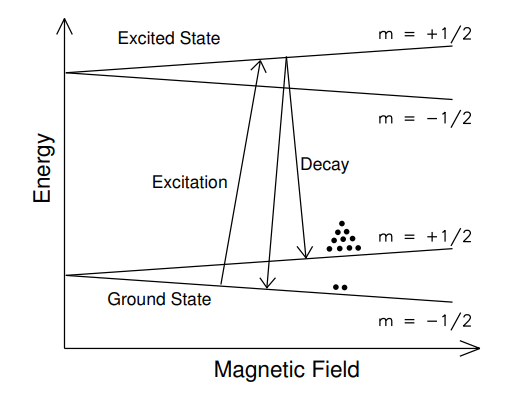
\includegraphics[width=0.7\textwidth]{images/optisches_pumpen.png}
    \caption{Schematische Darstellung des Mechanismus des optischen Pumpens. \cite{optical_pumping_princeton}}
    \label{fig:optisches_pumpen}
\end{figure}

\subsection{Optisches Pumpen bei Rubidium}
\label{subsec:Rubidium}

Rubidium besitzt zwei Isotope, $\ce{^{85}Rb}$ und $\ce{^{87}Rb}$ mit Kernspins $I = 5/2$ und $I = 3/2$. Es gehört zur Alkalimetallgruppe und besitzt somit nur ein Elektron in der äußersten Schale.
Wie in \autoref{subsec:Drehimpuls} beschrieben, gibt es verschiedene Energieaufspaltungen. Diese sind für Rubidium in \autoref{fig:rubidium} dargestellt.

\begin{figure}[H]
    \centering
    \begin{subfigure}[b]{0.45\textwidth}
        \centering
        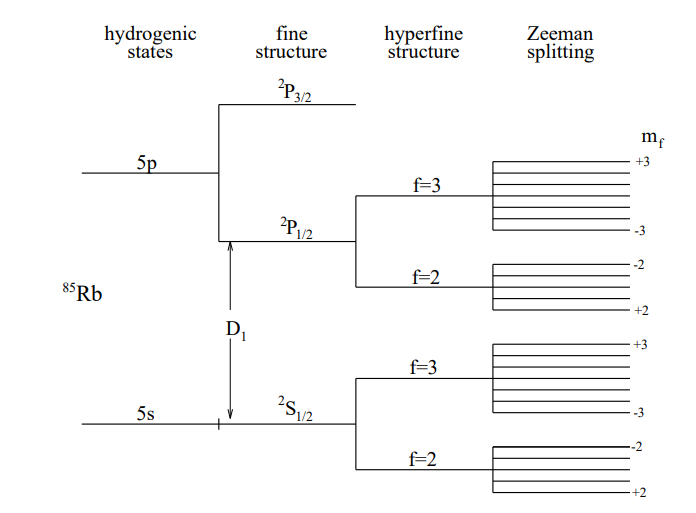
\includegraphics[height=0.3\textheight]{images/rub85.png}
        \caption{Aufspaltung der Energieniveaus von $\ce{^{85}Rb}$.}
        \label{fig:rubidium_85}
    \end{subfigure}
    \hfill
    \begin{subfigure}[b]{0.45\textwidth}
        \centering
        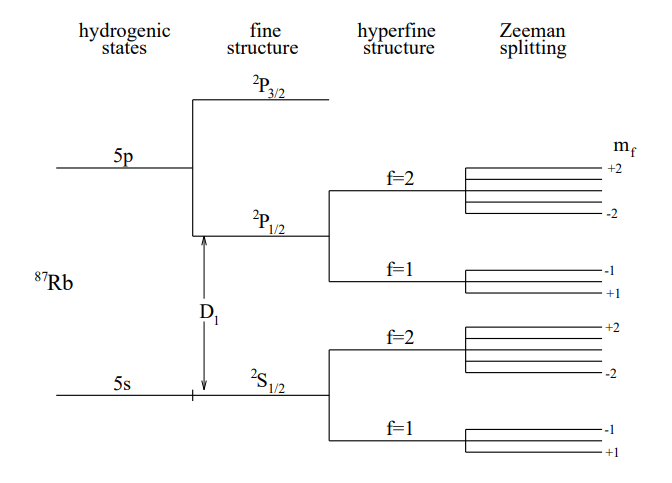
\includegraphics[height=0.3\textheight]{images/rub87.png}
        \caption{Aufspaltung der Energieniveaus von $\ce{^{87}Rb}$.}
        \label{fig:rubidium_87}
    \end{subfigure}
    \caption{Energieaufspaltung der Rubidium-Isotope. \cite{optical_pumping_princeton}}
    \label{fig:rubidium}
\end{figure}

Für niedrige Magnetfeldstärken ist die Energieaufspaltung linear im Magnetfeld $B$. Wenn der Zeeman-Effekt dominiert, müssen Terme höherer Ordnung berücksichtigt werden. Die Energiedifferenz ist dann
in quadratischer Ordnung gegeben durch
\begin{equation*}
    \Delta E = -\epsilon g_I \pm \frac{\Delta}{2} \cdot \bigg( \frac{2w}{2I+1} + \frac{2w^2(1-2m_F)}{(2I+1)^2}\bigg).
\end{equation*}
Dabei ist $\epsilon = \frac{e\hbar}{2m_e}B$, $w = \frac{\epsilon(g_J + g_I)}{\Delta}$ und $m_F = m_I \pm \frac{1}{2}$. Das grundlegende Prinzip des optischen Pumpens wurde bereits in \autoref{subsec:Mechanismus} erläutert.
Nun lässt sich an dem $\ce{^{87}Rb}$-Isotop konkret zeigen, wie optisches Pumpen in dem Versuch funktioniert.\\
Wenn $\sigma^+$-Licht auf das Isotop trifft, gilt für die Auswahlregeln $\Delta m_J = +1$ bzw. $\Delta m_F = +1$. Da es keine Niveaus mit $m_F = 3$ gibt, sind die Elektronen im $m_F = 2$ Niveau
"gefangen". Wenn jetzt wieder die Bedingung für die Relaxationszeit erfüllt ist, wird das Niveau $m_F = 2$ des $\ce{^{2}S_{1/2}}$-Grundzustands gepumpt.\\
Durch das Pumpen nimmt die Absorption des Lichts ab und die Transmission des Lichts nimmt zu. Die Transmission ist also ein Maß für die Besetzung des $m_F = 2$ Niveaus.\\
Wenn nun die Transmission in Abhängigkeit eines äußeren Magnetfelds betrachtet wird, muss zunächst das Erdmagnetfeld kompensiert werden. 
Um die Besetzungsinversion auszugleichen, wird ein Hochfrequenzfeld angelegt, das die Elektronen aus dem gepumpten Zustand relaxieren lässt. Die Transmission nimmt wieder ab, da mehr Licht
absorbiert wird.\\
Mit dem Hochfrequenzfeld kann auch eine Resonanz erzeugt werden. Dies ist durch einen Peak in der Absorption erkennbar. Die Resonanzbedingung ist gegeben durch
\begin{equation*}
    h \cdot f = g_F \cdot \mu_{\text{B}} \cdot B.
\end{equation*}


\newpage
